% 依试点教材文科固定来源第 1 页四种函数图象选项转绘；拓扑示意，不表示精确比例。
\begin{center}
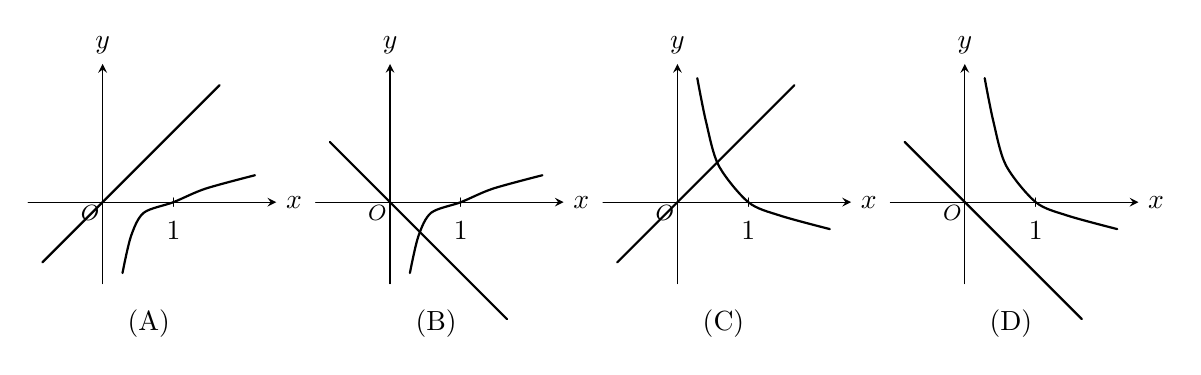
\begin{tikzpicture}[x=0.9cm,y=0.9cm,>=stealth,line cap=round,line join=round]
\foreach \xshift/\label/\lineup/\logup in {0/A/1/1,3.65/B/-1/1,7.3/C/1/-1,10.95/D/-1/-1} {
  \begin{scope}[xshift=\xshift cm]
    \draw[->] (-1.05,0)--(2.45,0) node[right] {$x$};
    \draw[->] (0,-1.15)--(0,1.95) node[above] {$y$};
    \draw (1,0.06)--(1,-0.06) node[below=2pt] {$1$};
    \node[below left,font=\footnotesize,inner sep=1pt] at (0,0) {$O$};
    \ifnum\lineup=1
      \draw[thick] (-0.85,-0.85)--(1.65,1.65);
    \else
      \draw[thick] (-0.85,0.85)--(1.65,-1.65);
    \fi
    \ifnum\logup=1
      \draw[thick] plot[smooth] coordinates {(0.28,-1.0) (0.4,-0.48) (0.58,-0.15) (1,0) (1.45,0.19) (2.15,0.38)};
    \else
      \draw[thick] plot[smooth] coordinates {(0.28,1.75) (0.4,1.15) (0.58,0.52) (1,0) (1.45,-0.19) (2.15,-0.38)};
    \fi
    \node[below] at (0.65,-1.38) {(\label)};
  \end{scope}
}
\end{tikzpicture}
\end{center}
